\chapter{Solução Proposta}
\label{ch:4}

Neste capítulo, apresentaremos os componentes desenvolvidos para a realização dos objetivos propostos, bem como, detalhes de implementação considerados importantes para o melhor entendimento técnico do mecanismo. 

Também será mostrada uma análise do processo de gerenciamento automático, tendo em vista as ideias do ciclo PDCA apresentado na Seção \ref{sec:pdca} deste trabalho. Essa análise irá relacionar as etapas definidas no ciclo com os sub-processos definidos pelo mecanismo.

\section{Visão Geral}
Como foi dito no Capítulo \ref{ch:1}, a proposta deste trabalho é especificar e construir um mecanismo de gerenciamento automático de provedores de serviço, focado na prevenção de possíveis quebras de contrato.

O contexto ao qual este trabalho está inserido, foi apresentado no capítulo \ref{ch:3}, através da plataforma DSOA, ver Seção \ref{sec:dsoa_arch}, que provê um ambiente de composição dinâmica baseado em componentes orientados a serviços, com percepção de requisitos não-funcionais mapeados em atributos de qualidade.

Neste trabalho foi desenvolvido um módulo de monitoração de recursos de hardware, instrumentado através de JMX e disponibilizado como um serviço da plataforma. 

Outro módulo criado neste trabalho, é o módulo de gerenciamento de provedor do serviço, ele define um \textit{container} com suporte a reconfiguração dinâmica de serviços com base em atributos de qualidade e no contexto em que o provedor executa.

A figura \ref{fig:proposal} destaca onde o trabalho desenvolvido esta situado na plataforma DSOA.

\begin{figure}[htp]
\centering
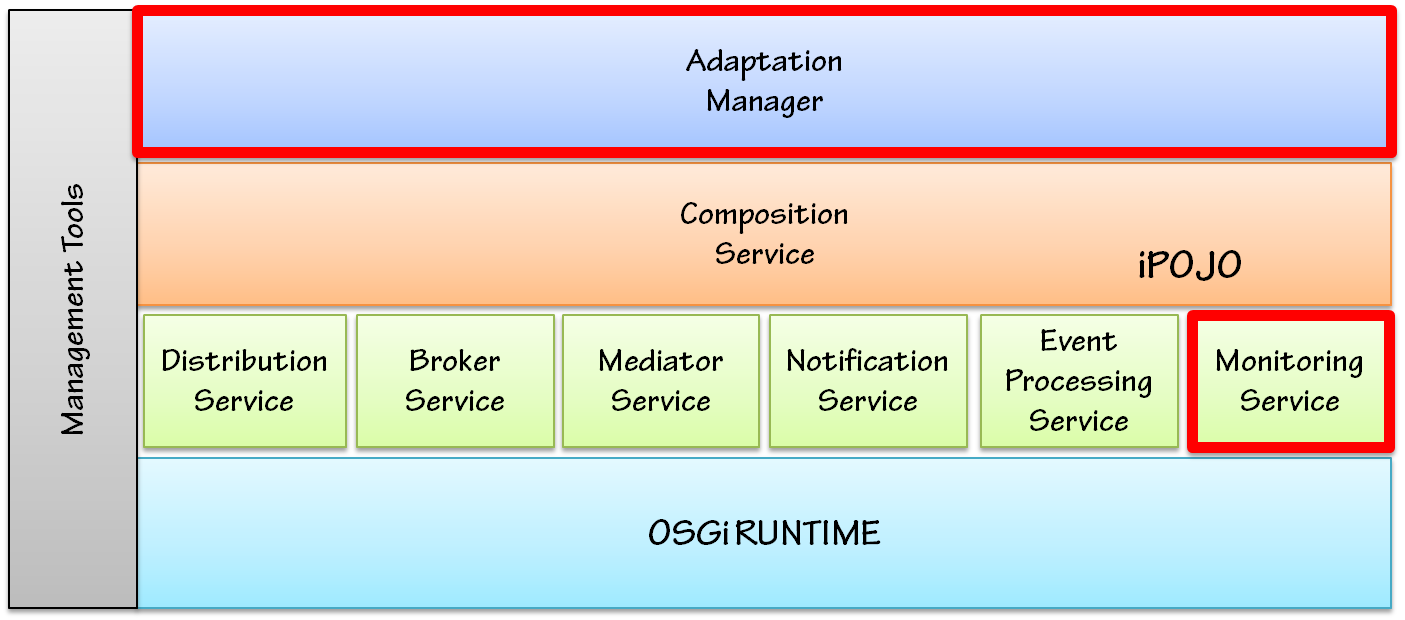
\includegraphics[width=12cm]{chapters/chapter4/dsoa-provider-manager.png}
\caption[Visão Geral da Proposta na Arquitetura]{Visão Geral da Proposta na Arquitetura.}
\label{fig:proposal}
\end{figure}

Todo o processo de monitoramento e adaptação será baseado nas etapas definidas pelo ciclo PDCA. 

Na etapa de planejamento, as metas serão definidas por meio de um documento XML~\cite{xml} que descreve as capacidades que o provedor afirma garantir. Essas propriedades são utilizadas para definir configurações de monitoramento (~\textit{Monitoring Configuration}) relacionadas a atributos de qualidade do provedor (\textit{e.g} tempo de processamento).

Além disso, 

\section{Arquitetura}
%TODO explicar arquitetura
